\documentclass[../TST.tex]{subfiles}
\begin{document}
\begin{eproblem}[Induction brake]{\ \\[5pt]}
\textit{Introduction:}\\
A permanent magnet moving along a non-magnetic metal surface will induce eddy currents in the metal. These give rise to a magnetic field that results in a drag force $\mathbf{F}$ on the magnet:
\begin{equation*}
\mathbf{F}=-k\mathbf{v}
,
\end{equation*}
where $\mathbf{v}$ is the velocity of the magnet and $k$ is the magnetic drag coefficient. This coefficient depends on the shape and size of the magnet, the magnetic field of the magnet, and the conductivity of the metal surface. The aim of this problem is to find $k$ for a magnet moving along an inclined aluminium surface.\\

\textit{Equipment:}
\begin{enumerate}
	\item Aluminium rail with U-shaped cross section (Figure \ref{fig1}).
	\item Neodymium magnet of mass $\qty{5.6}{g}$ in the shape of a rectangular cuboid. It is magnetised parallel to its shortest edge, i.e. its poles are on its largest surfaces.
	\item Stopwatch.
	\item Plastic tape measure, accurate to $\qty{1}{mm}$.
	\item Pencil.
	\item Ball of plasticine.
	\item Ruler.
	\item Blank paper and two sheets of graph paper.
\end{enumerate}
\textbf{Note:} The magnet is made from a brittle alloy and will easily break if struck. Take care not to break it.\\
\begin{figure}[h]
\centering
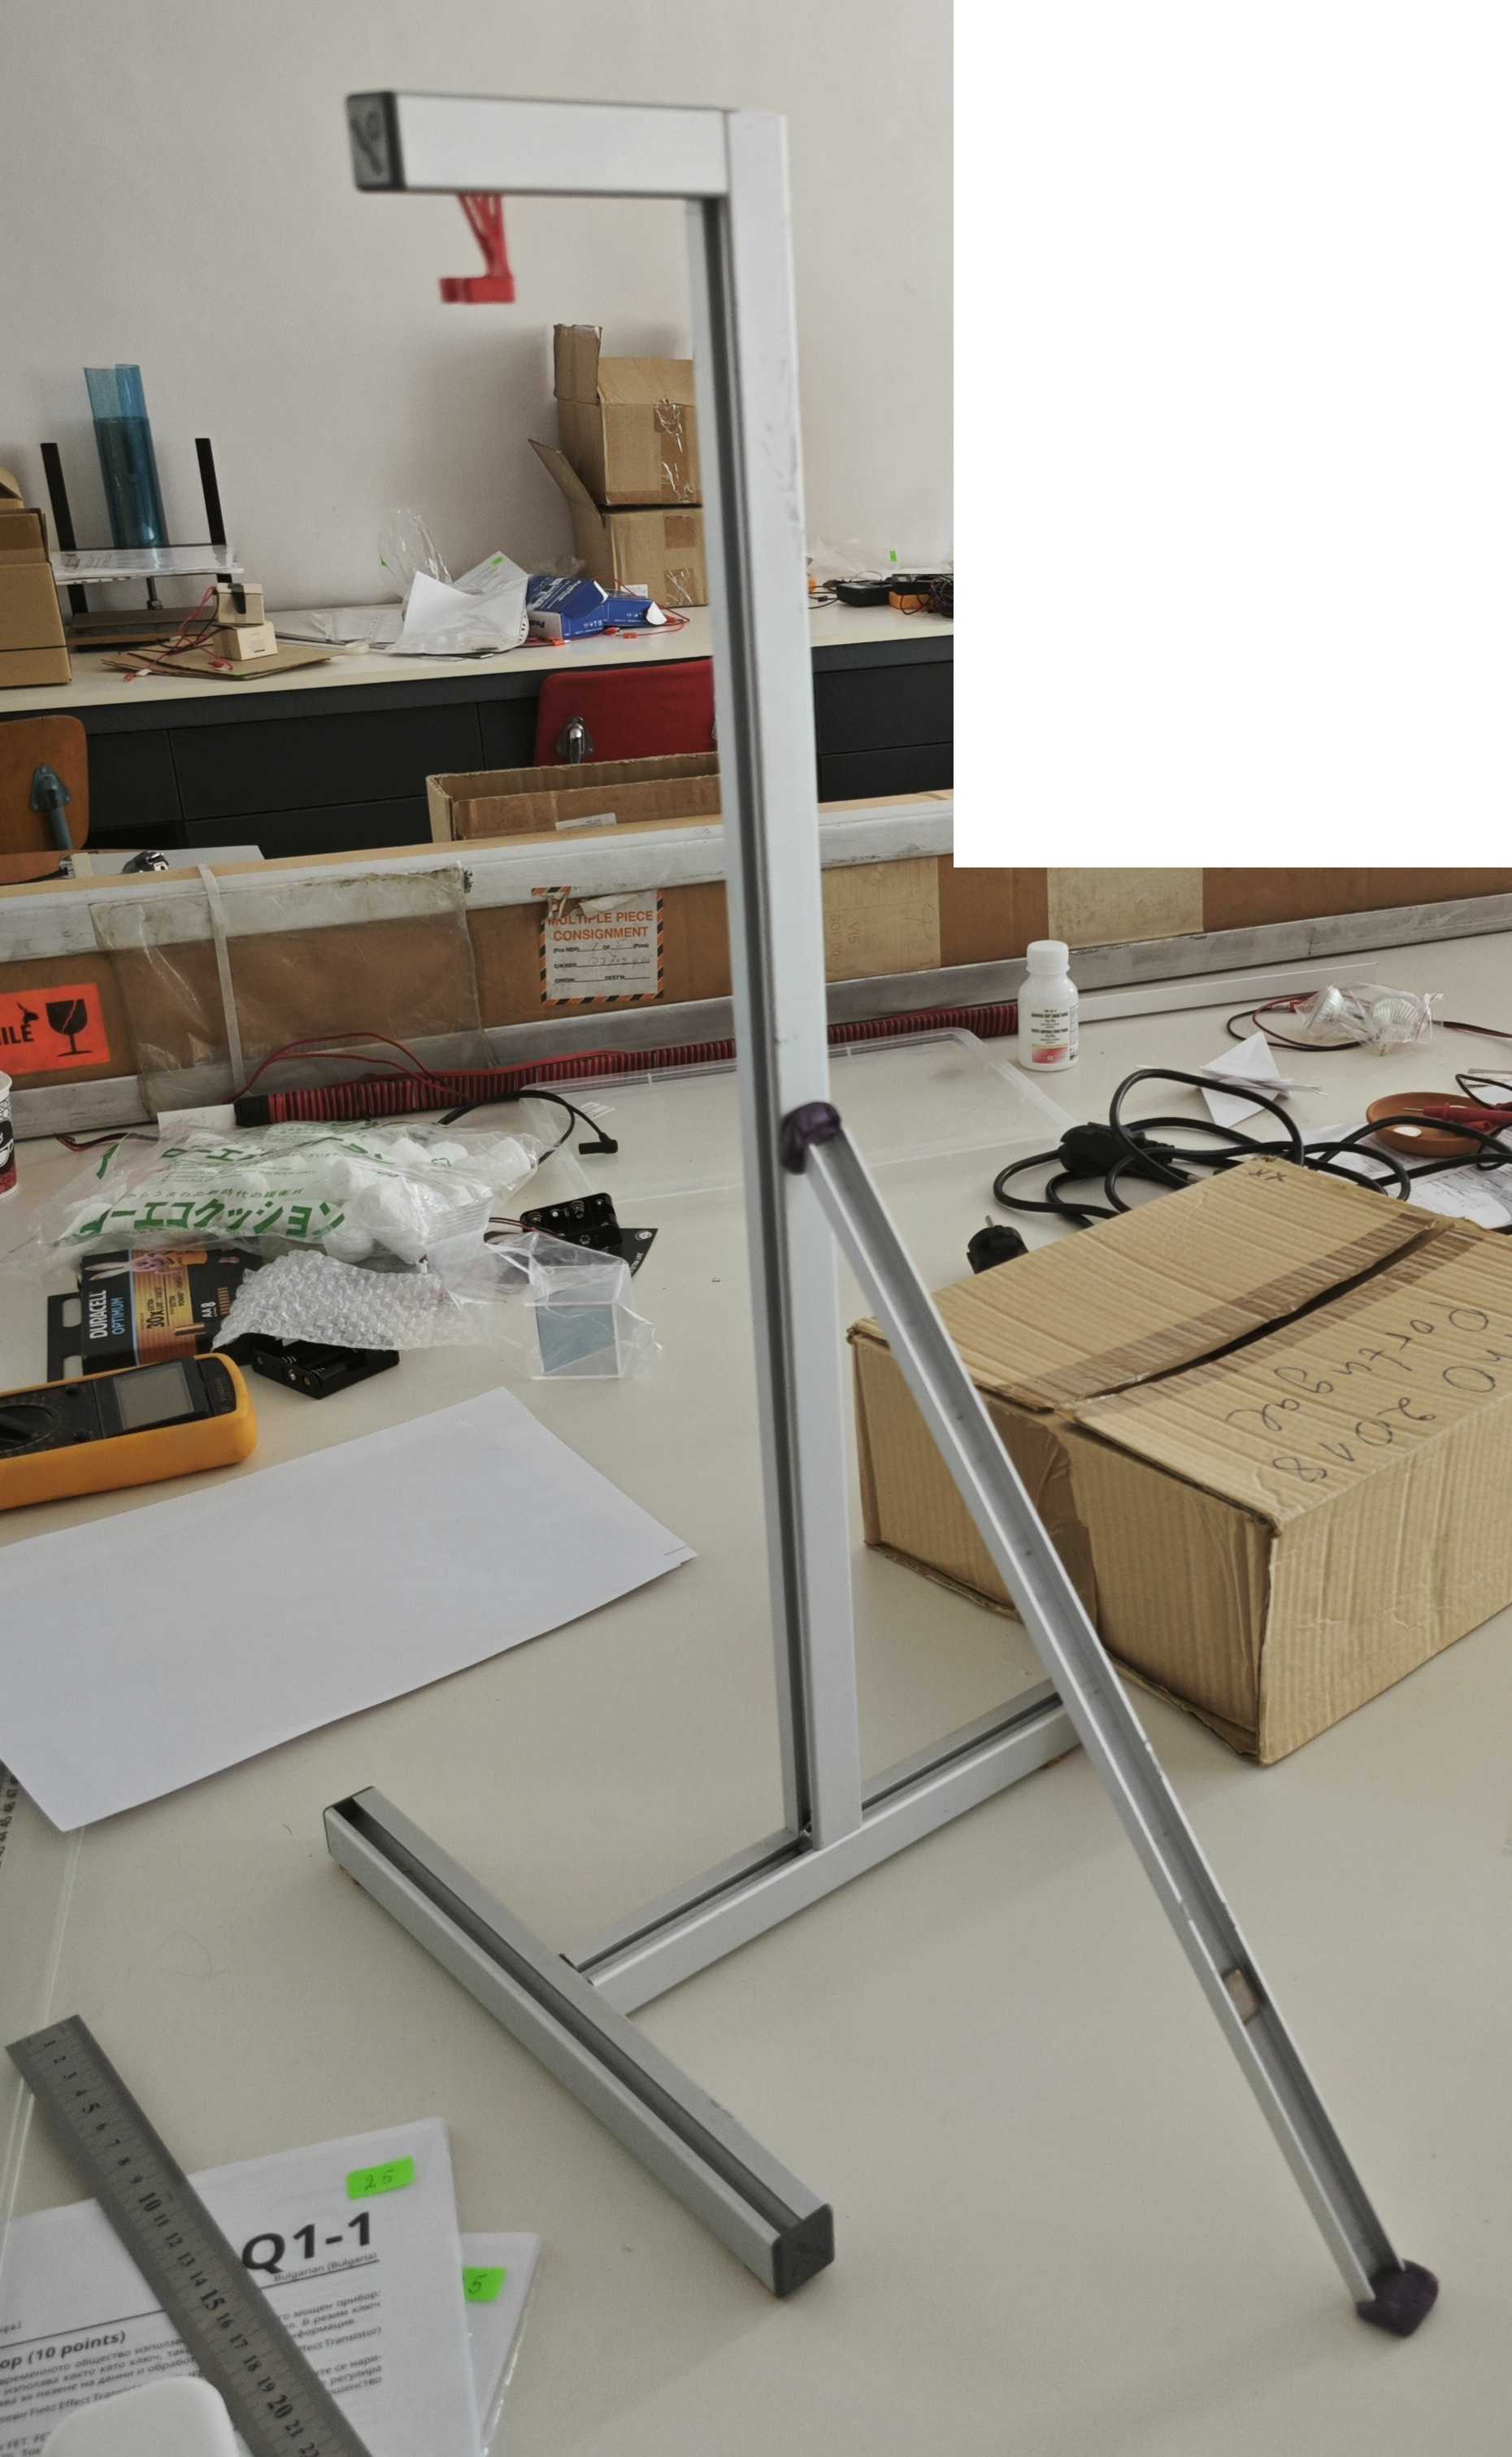
\includegraphics[width=0.39\textwidth]{fig/2013_e2.jpg}
\caption{}
\label{fig1}
\end{figure}

\textit{Tasks:}
\begin{subpart}
\item Write down the equation of motion for a magnet on a metal surface at an angle $\alpha$ to the horizon. The magnetic drag coefficient is $k$ and the coefficient of dynamic friction is $\mu$. Find an expression for the terminal velocity of the magnet $v_\mathrm{t}$ assuming the rail is long enough.
\item Place the rail an an angle of $\ang{60}$ to the horizontal table. Explain how you have found the angle. You can affix the lower end of the rail to the plasticine and lean the upper end on the wall. Place the magnet with one of its poles lying on the aluminium surface. Let the magnet slide with zero initial velocity from different initial heights. Study the dependence of distance moved $s$ against time $t$. Present your data in tabular and graphical form.
\item Analyse the graph from (b). State the type of motion within the time intervals you worked with. Find the terminal velocity of this motion $v_\mathrm{t}$.
\item Study the descent of the magnet at different slopes $\alpha<\ang{60}$ (though large enough for the magnet to slide). Find the terminal velocity $v_\mathrm{t}$ for each of the angles $\alpha$. Present your results in a table.
\item Find auxiliary variables $x$ and $y$ (expressed in terms of the slope $\alpha$ and the terminal velocity $v_\mathrm{t}$) for which a linear dependence is expected. Present your data in terms of these variables in tabular and graphical form. Using your graph, find the coefficient of dynamic fricion $\mu$ and the magnetic drag coefficient $k$.
\item The time dependence for the velocity of the magnet is given by
	\begin{equation}
		v(t)=v_\mathrm{t}(1-e^{-t/\tau})
	,
	\label{vel}
	\end{equation}
	where $\tau$ is a time constant which is independent of the slope (that is, the time taken to reach $\qty{63.2}{\percent}$ of the terminal velocity). Using your data, find the time constant $\tau$. Is it possible to verify Equation \eqref{vel} experimentally using only the equipment given?  
\end{subpart}
\end{eproblem}
\end{document}
